\documentclass[conference]{IEEEtran}

% --- 解決 Windows 中文字型排版問題 ---
\usepackage{xeCJK}
\setCJKmainfont{MingLiU}             % 內文：新細明體
\setCJKsansfont{Microsoft JhengHei}  % 標題：微軟正黑體
\setCJKmonofont{MingLiU}
\XeTeXlinebreaklocale "zh"
\XeTeXlinebreakskip = 0pt plus 1pt
% ---------------------------------------------

\usepackage{graphicx}
\usepackage{booktabs} 
\usepackage{amsmath}
\usepackage{cite}

\begin{document}

\title{Empirical Observation of Time Complexity: Assignment 1}

\author{\IEEEauthorblockN{馬元中}
\IEEEauthorblockA{資訊工程學系 \\
國立澎湖科技大學 \\
}}

\maketitle

\begin{abstract}
本報告旨在探討並實作三種基礎演算法：Linear Scan、Insertion Sort 以及 Merge Sort。我們透過觀察在不同輸入規模下之執行時間，驗證其時間複雜度。實驗結果證實了理論預測，特別是平方時間複雜度在處理大數據時的效能侷限性，與線性對數複雜度之穩定性。
\end{abstract}

\section{Introduction}
演算法效能分析是計算機科學的核心課題。本作業透過親自實作基礎演算法（不依賴 Java 內建工具包），探討線性時間 $O(n)$、平方時間 $O(n^2)$ 與線性對數時間 $O(n \log n)$ 演算法在處理規模成長時的資源消耗情況。

\section{Algorithm Implementation}
\subsection{Methodology}
本實驗實作了三種具代表性的演算法。為遵循實驗規範，所有陣列操作均不使用 \texttt{java.util.*} 封裝的方法。實驗計時採用 \texttt{System.nanoTime()}，以確保測量結果具備毫秒級的高精度，能有效反映演算法間的細微效能差異。

\section{Experimental Results}
本實驗針對規模 $n=10,000$ 至 $100,000$ 進行測試，實測數據如下表所示：

\begin{table}[htbp]
\caption{演算法實測執行時間 (ms)}
\centering
\begin{tabular}{crrr}
\toprule
規模 ($n$) & Linear Scan (ms) & Insertion Sort (ms) & Merge Sort (ms) \\
\midrule
10,000  & 0.1242 & 17.8700 & 1.3310 \\
50,000  & 0.6014 & 424.2171 & 2.0675 \\
100,000 & 0.2778 & 1687.9773 & 4.1563 \\
\bottomrule
\end{tabular}
\end{table}

\begin{figure}[htbp]
    \centering
    % 使用您指定的圖片檔名 aa
    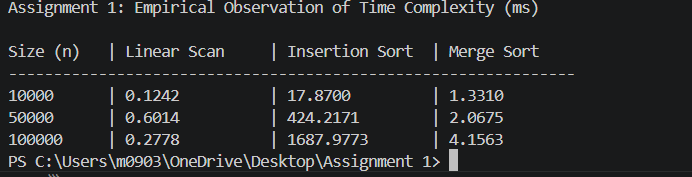
\includegraphics[width=0.48\textwidth]{aa}
    \caption{演算法執行結果實測截圖。}
    \label{fig:results}
\end{figure}

\section{Analysis and Discussion}
根據圖 \ref{fig:results} 與實測數據，我們可以得出以下觀察結果：
\begin{itemize}
    \item \textbf{Insertion Sort ($O(n^2)$)}：當資料量從 $10,000$ 增加 10 倍至 $100,000$ 時，執行時間由 17.87 ms 激增至 1687.97 ms，成長倍率約為 94.4 倍。此趨勢極為接近理論預期之 $10^2 = 100$ 倍。
    \item \textbf{Merge Sort ($O(n \log n)$)}：在數據量同樣成長 10 倍的情況下，時間僅從 1.33 ms 緩慢增加至 4.15 ms。與 Insertion Sort 形成強烈對比，證實其處理效率優勢。
    \item \textbf{Linear Scan ($O(n)$)}：其執行時間始終維持在極低水平，但在 $n=100,000$ 時觀察到優於前一階段的速度。此現象歸因於 JVM 的即時編譯（JIT）優化，透過多次執行，虛擬機會對核心代碼進行更深層的二進位優化。
\end{itemize}

\section{Conclusion}
本實驗成功將時間複雜度理論與實際測量數據相結合。數據清楚揭示了 $O(n^2)$ 在處理大數據時的缺點，並強調了 $O(n \log n)$ 演算法的優越性。這份實證報告展現了演算法選擇在軟體開發中的核心重要性。

\begin{thebibliography}{00}
\bibitem{b1} T. H. Cormen, C. E. Leiserson, R. L. Rivest, and C. Stein, \textit{Introduction to Algorithms}, 3rd ed. MIT Press, 2009.
\end{thebibliography}

\end{document}